% !TeX program = xelatex
% !TeX root = design_presentation.tex
\documentclass[UTF8,aspectratio=169]{ctexbeamer}

\usepackage{zju}
\usepackage{amsmath}
\usepackage{booktabs}
\usepackage{graphicx}
\usepackage{hyperref}
\usepackage{xcolor}
\usepackage{tikz}

\graphicspath{
    {./}
    {../figures/}
    {../figures/exported/}
    {../figures/ui/}
    {docs/总体设计报告/presentation/}
    {docs/总体设计报告/figures/}
    {docs/总体设计报告/figures/exported/}
    {docs/总体设计报告/figures/ui/}
}

\beamertemplateballitem
\setbeamertemplate{navigation symbols}{}
\setbeamerfont{frametitle}{size=\large,series=\bfseries}
\setbeamerfont{itemize/enumerate body}{size=\small}
\setbeamerfont{itemize/enumerate subbody}{size=\footnotesize}
\setbeamerfont{block body}{size=\small}
\setbeamerfont{caption}{size=\scriptsize}
\definecolor{ZJUBlue}{RGB}{0,63,136}
\definecolor{SoftGray}{RGB}{245,247,250}

\title[总体设计报告展示]{校园学术活动智能推荐平台}
\subtitle{总体设计报告汇报}
\author[SE 第 4 组]{黄晗 \quad 宫上珺 \quad 孟祥烨 \\ 李妍雅 \quad 庞星磊 \quad 朱致远}
\institute[浙江大学]{}
\date[2026-05]{2026 年 5 月}

\newcommand{\keyword}[1]{\textcolor{ZJUBlue}{\textbf{#1}}}
\newcommand{\imgfit}[2]{\includegraphics[width=#1\linewidth,height=#2\textheight,keepaspectratio]{#2}}

\begin{document}

\begin{frame}
    \titlepage
\end{frame}

\section{项目定位}
\begin{frame}{项目定位：把分散活动整理为个人日程}
    \begin{columns}[T,onlytextwidth]
        \begin{column}{0.48\textwidth}
            \begin{block}{现有问题}
                \begin{itemize}
                    \item 活动发布在不同学院网站，学生需要反复查找
                    \item 活动数量增加后，单纯按时间浏览效率较低
                    \item 是否与课程冲突通常要人工对照课表
                    \item 手工录入和爬虫数据需要一个维护入口
                \end{itemize}
            \end{block}
        \end{column}
        \begin{column}{0.48\textwidth}
            \begin{block}{系统设计目标}
                \begin{itemize}
                    \item 统一管理爬虫采集和后台录入的活动数据
                    \item 支持关键词检索、条件筛选和基础排序
                    \item 基于兴趣标签生成可解释的活动推荐
                    \item 在加入日程前检查课程和已有安排的时间冲突
                \end{itemize}
            \end{block}
        \end{column}
    \end{columns}
\end{frame}

\section{总体架构}
\begin{frame}{总体架构：B/S、前后端分离与后端分层}
    \begin{columns}[T,onlytextwidth]
        \begin{column}{0.56\textwidth}
            \centering
            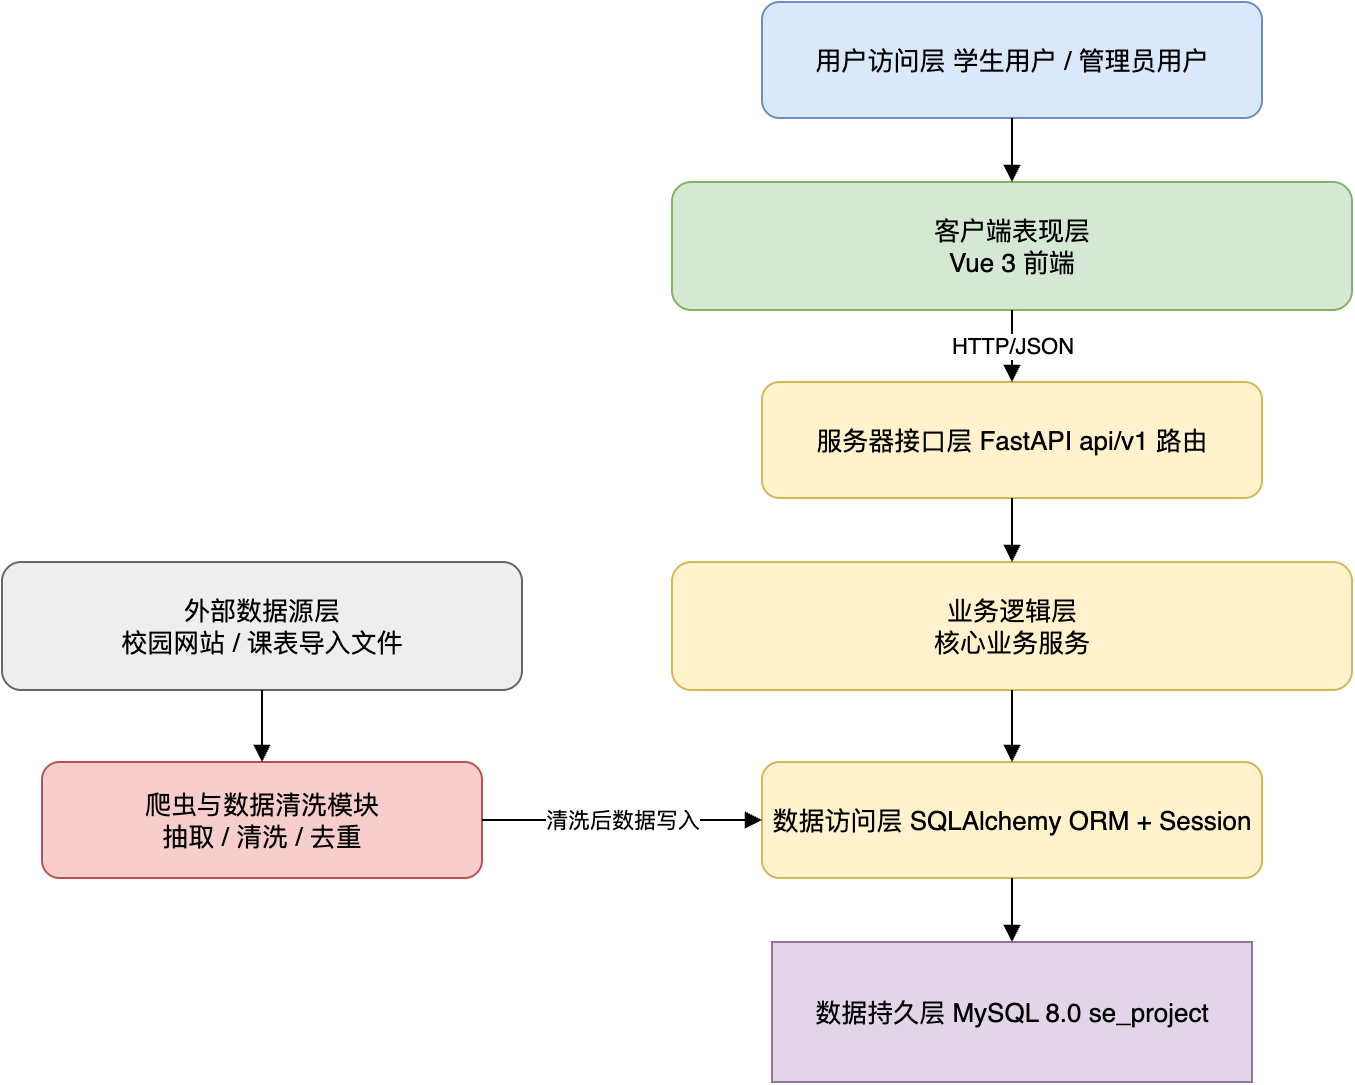
\includegraphics[width=\linewidth,height=0.62\textheight,keepaspectratio]{1.3-系统层级结构.png}
        \end{column}
        \begin{column}{0.40\textwidth}
            \begin{itemize}
                \item \keyword{客户端表现层}：负责页面展示、表单交互和路由跳转
                \item \keyword{服务器接口层}：接收请求，完成参数校验和响应封装
                \item \keyword{业务逻辑层}：处理活动查询、推荐计算和冲突检测
                \item \keyword{数据访问层}：用 ORM 访问 MySQL，屏蔽具体 SQL 细节
                \item \keyword{外部数据源}：校园网站、课表文件和日历工具
            \end{itemize}
        \end{column}
    \end{columns}
\end{frame}

\begin{frame}{后端设计：路由保持轻量，业务放在 Service 层}
    \begin{columns}[T,onlytextwidth]
        \begin{column}{0.52\textwidth}
            \centering
            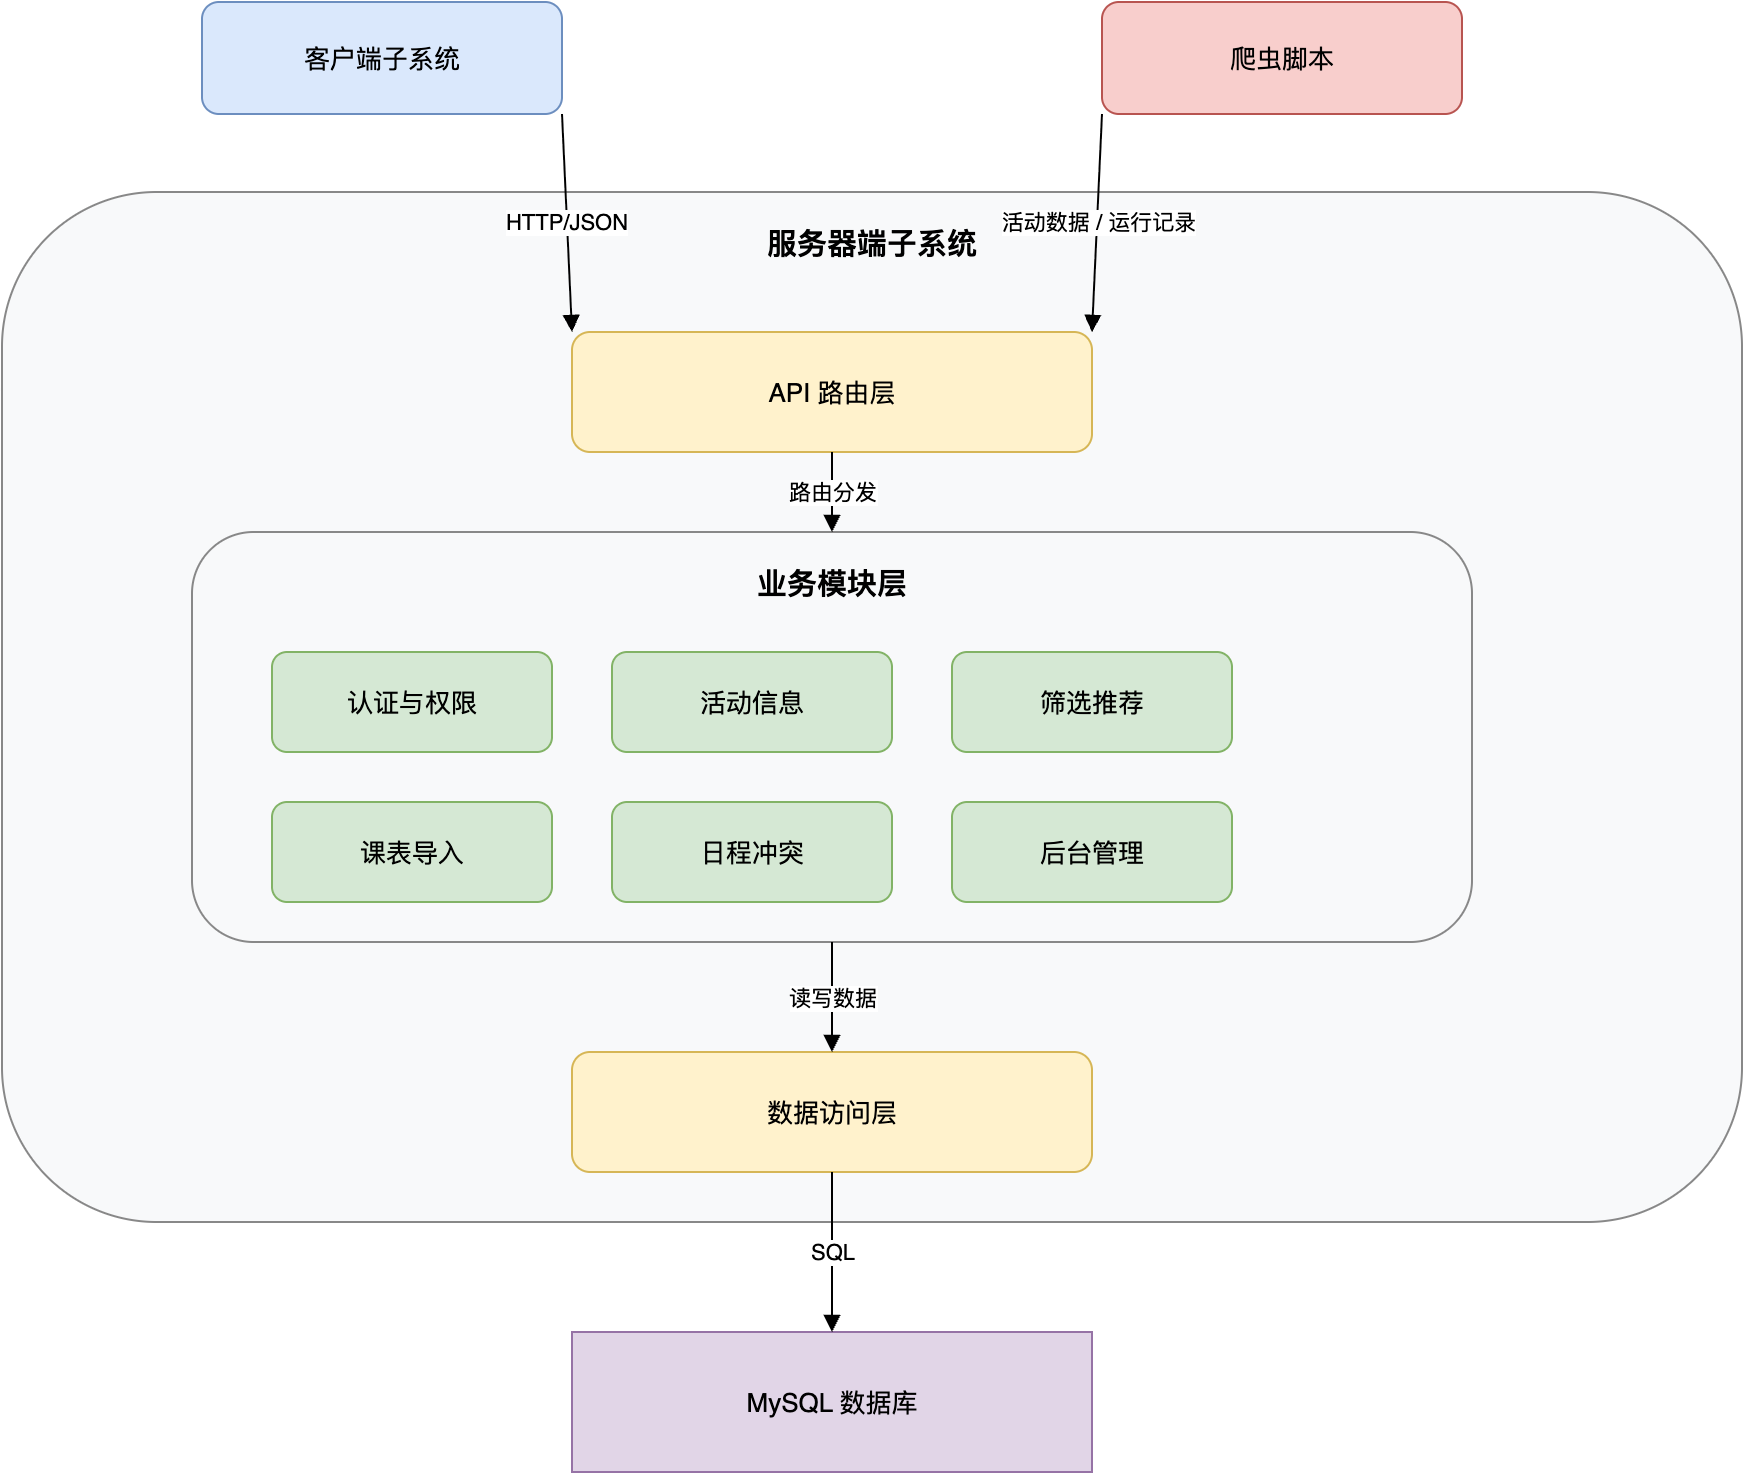
\includegraphics[width=\linewidth,height=0.9\textheight,keepaspectratio]{1.4.2-服务器端子系统.png}
        \end{column}
        \begin{column}{0.44\textwidth}
            \begin{block}{分层约束}
                \begin{itemize}
                    \item 路由层只处理参数、依赖注入、权限和响应格式
                    \item Service 层集中实现查询组装、推荐计算和冲突检测
                    \item ORM 模型字段与 \texttt{schema.sql} 保持一致
                    \item 前端按统一响应结构判断请求结果：
                \end{itemize}
                \vspace{-0.4em}
                \[
                    \{code,\ message,\ data\}
                \]
            \end{block}
        \end{column}
    \end{columns}
\end{frame}

\section{核心流程}
\begin{frame}{推荐流程：先过滤候选活动，再按规则排序}
    \begin{columns}[T,onlytextwidth]
        \begin{column}{0.55\textwidth}
            \centering
            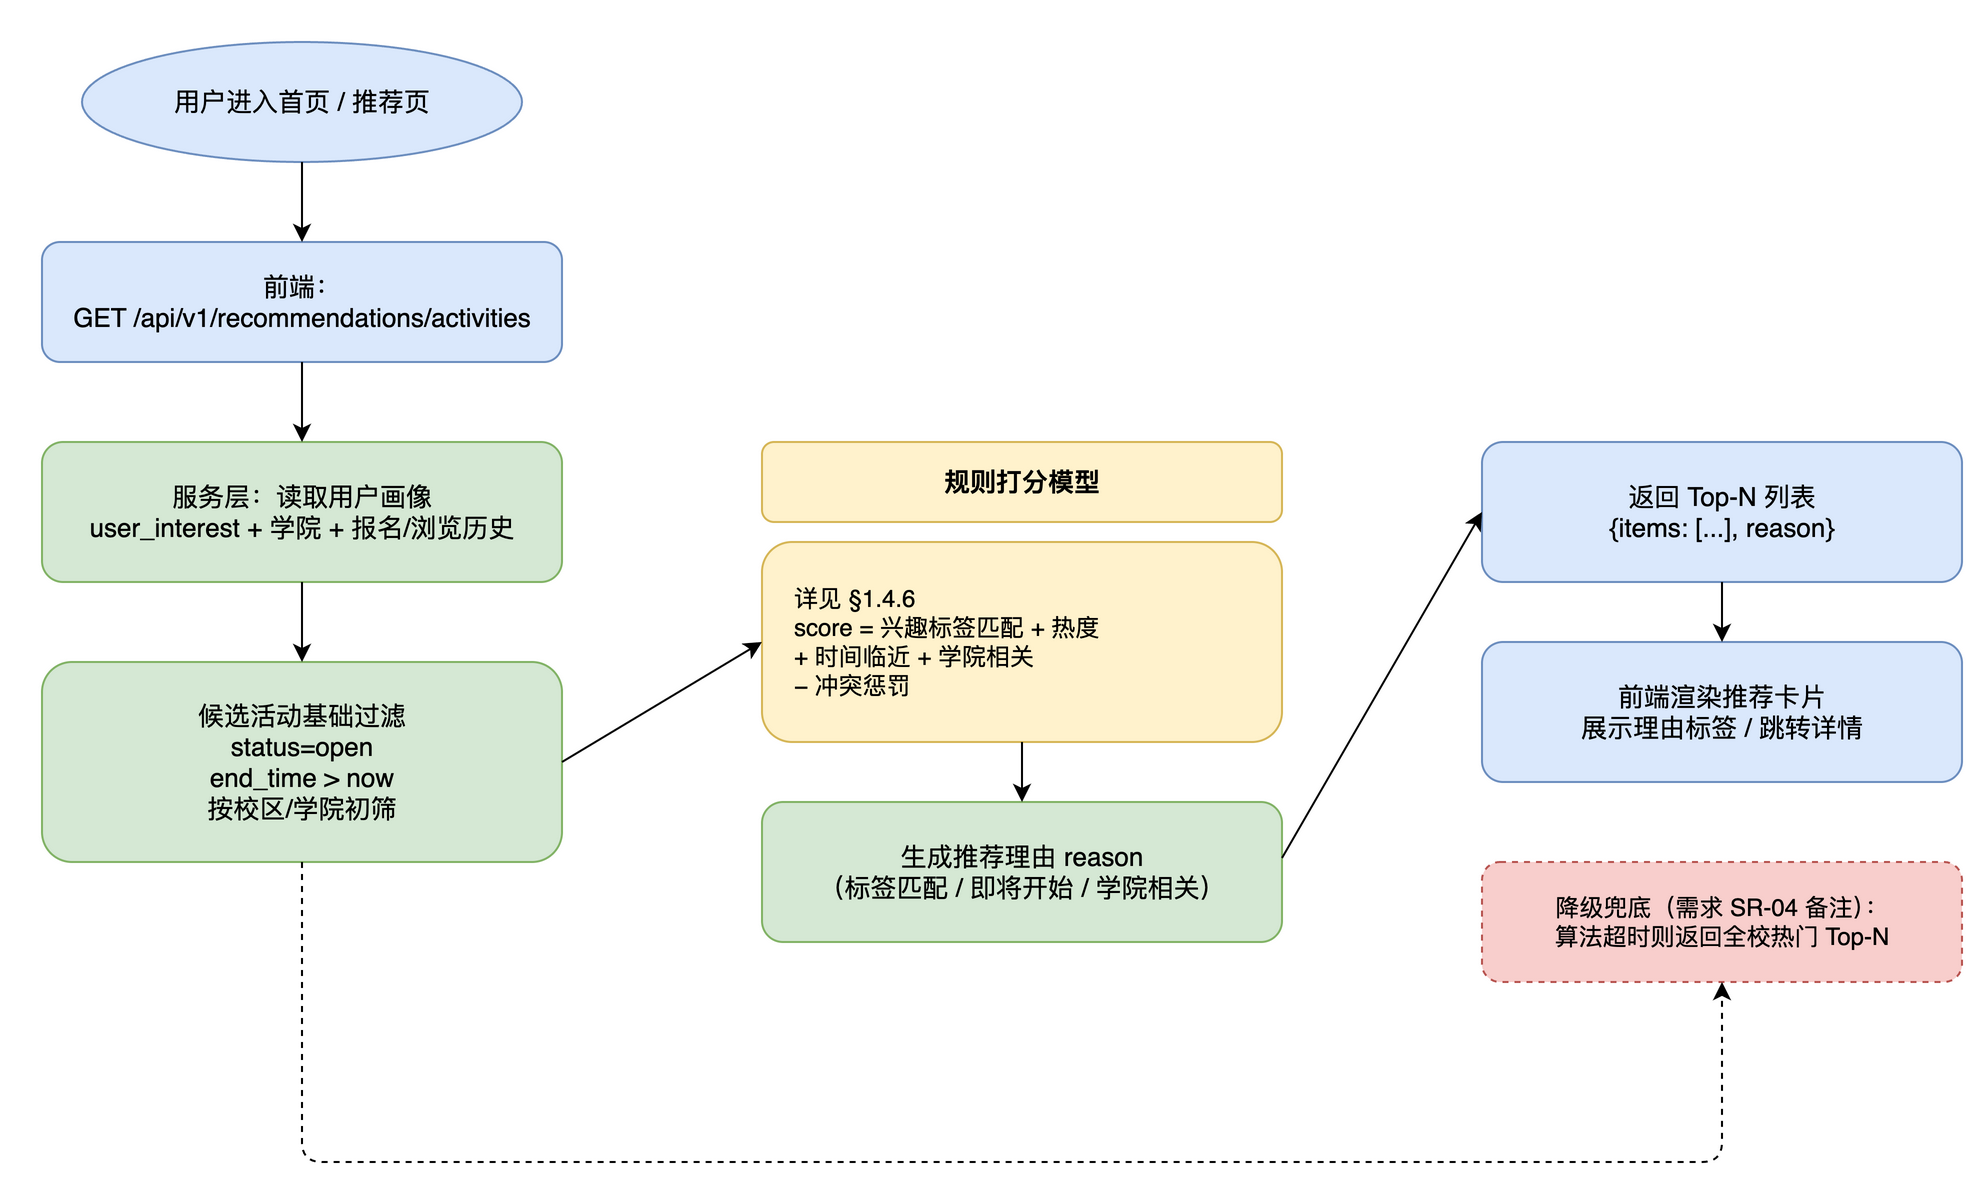
\includegraphics[width=\linewidth,height=0.8\textheight,keepaspectratio]{2.2.2-个性化推荐流程.png}
        \end{column}
        \begin{column}{0.41\textwidth}
            \begin{block}{第一阶段采用规则模型}
                \[
                    score = I + H + T + C - P
                \]
                \begin{itemize}
                    \item $I$：活动标签与兴趣标签匹配
                    \item $H$：活动热度
                    \item $T$：活动开始时间的临近程度
                    \item $C$：活动学院与用户学院相关性
                    \item $P$：课程或已有日程冲突扣分
                \end{itemize}
            \end{block}
        \end{column}
    \end{columns}
\end{frame}

\begin{frame}{日程流程：写入前检查时间区间重叠}
    \begin{columns}[T,onlytextwidth]
        \begin{column}{0.56\textwidth}
            \centering
            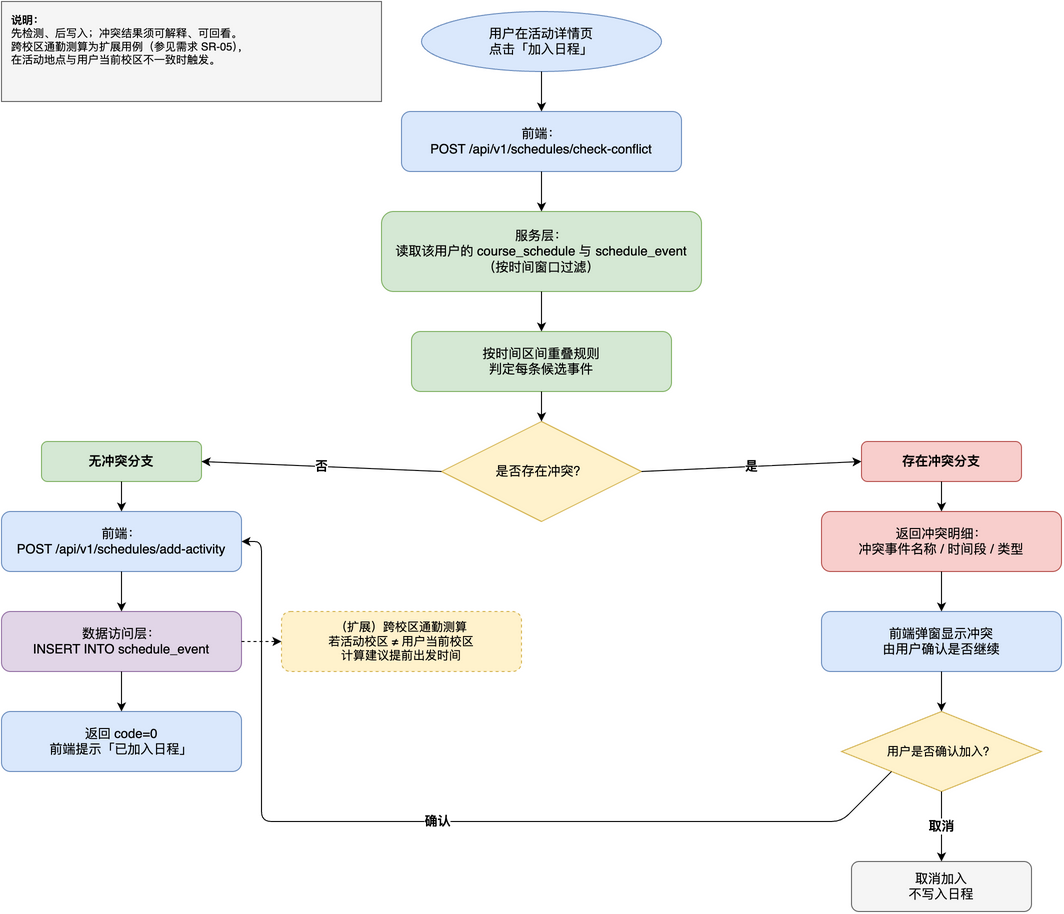
\includegraphics[width=\linewidth,height=0.9\textheight,keepaspectratio]{2.2.4-加入日程冲突检测流程.png}
        \end{column}
        \begin{column}{0.40\textwidth}
            \begin{itemize}
                \item 用户在活动详情页点击“加入日程”
                \item 后端读取该用户的课程表和已有日程
                \item 用活动起止时间与已有事件时间段比较
                \item 如果存在重叠，返回冲突事件和重叠时间
                \item 用户确认后再创建新的日程记录
            \end{itemize}
        \end{column}
    \end{columns}
\end{frame}

\section{数据与采集}
\begin{frame}{数据设计：以用户、活动和日程为主线}
    \begin{columns}[T,onlytextwidth]
        \begin{column}{0.54\textwidth}
            \centering
            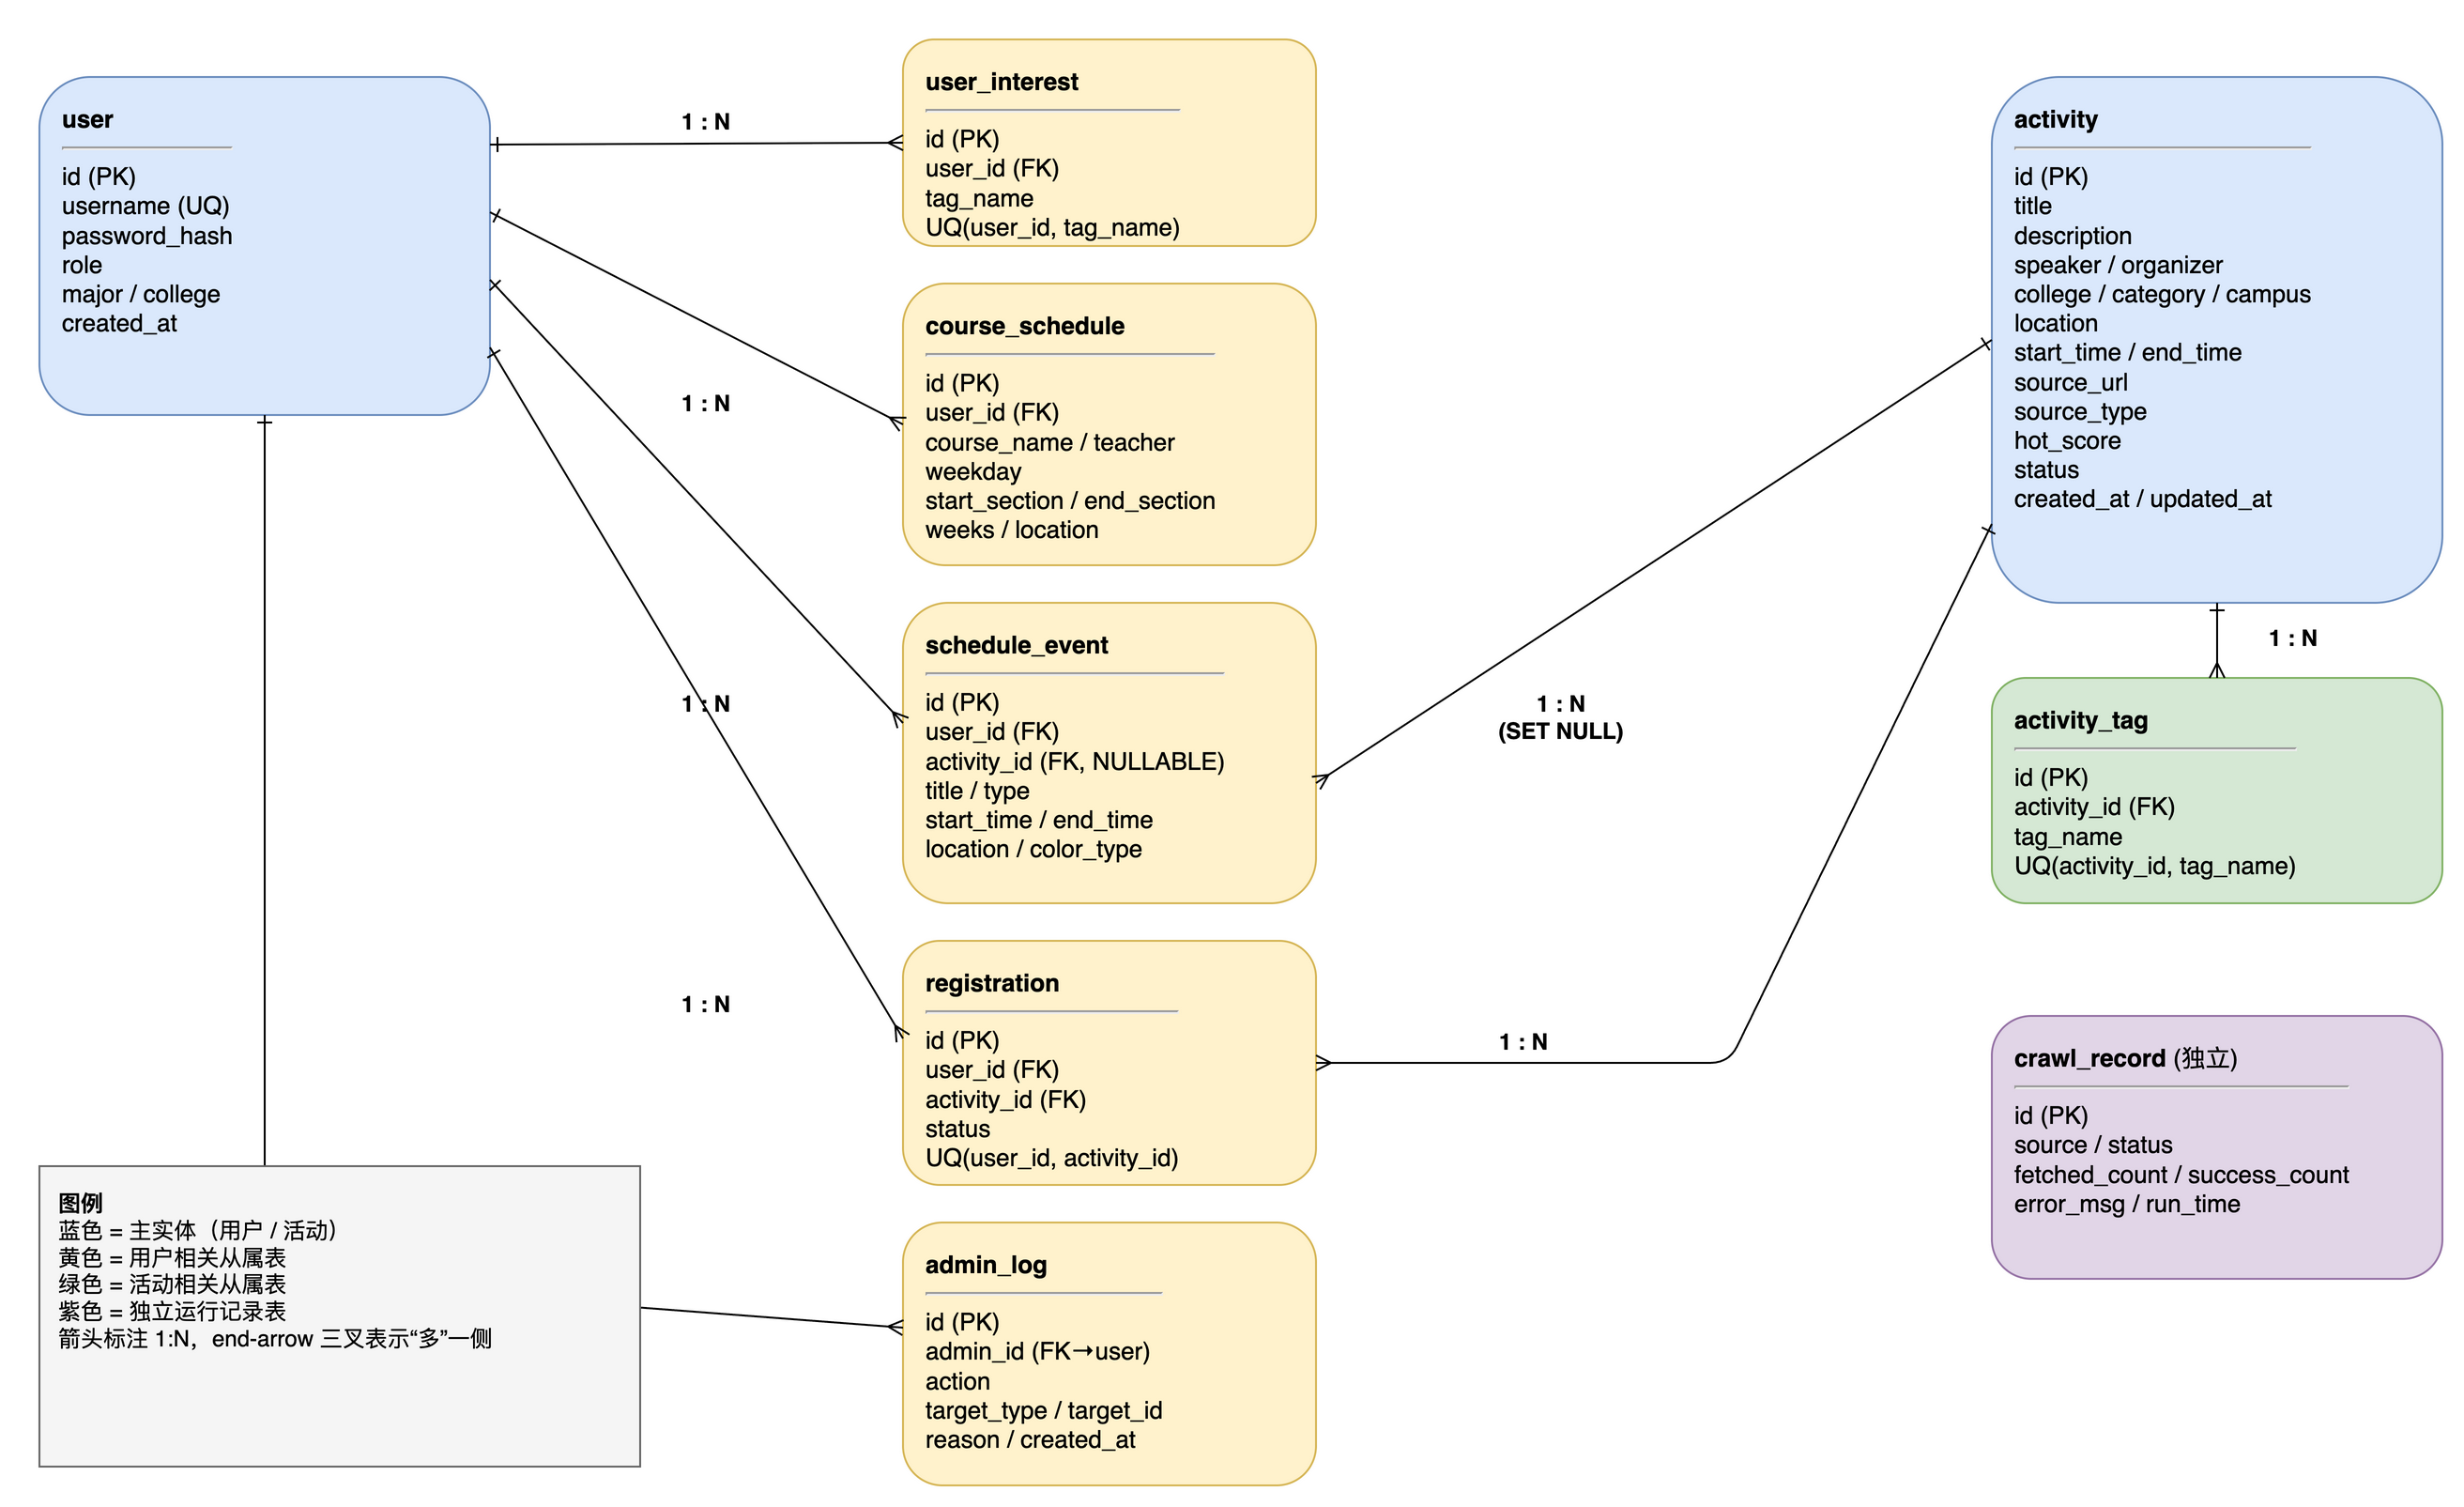
\includegraphics[width=\linewidth,height=0.9\textheight,keepaspectratio]{2.3.2-数据库ER图.png}
        \end{column}
        \begin{column}{0.44\textwidth}
            \begin{itemize}
                \item 数据库设计为 9 张核心表，避免把活动、课表和日志混在单表中
                \item \keyword{activity} 保存活动主信息，供列表、详情和推荐复用
                \item \keyword{activity\_tag} 与 \keyword{user\_interest} 提供推荐和筛选输入
                \item \keyword{schedule\_event} 保存已加入的活动和个人日程事件
            \end{itemize}
        \end{column}
    \end{columns}
\end{frame}

\begin{frame}{数据采集：从学院网站解析活动并入库}
    \centering
    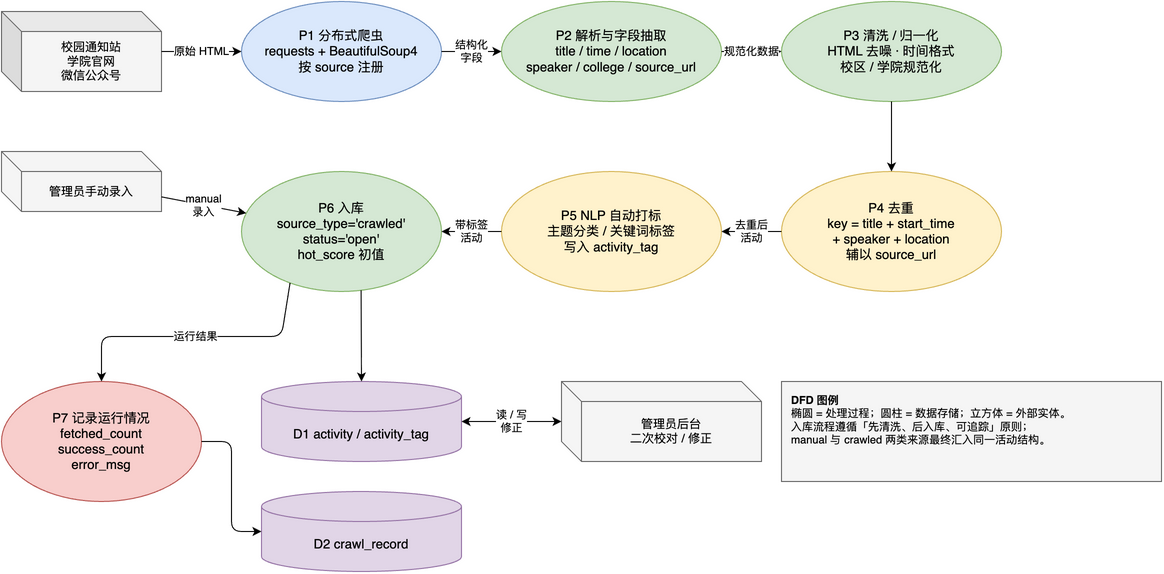
\includegraphics[width=0.92\linewidth,height=0.50\textheight,keepaspectratio]{2.5.1-数据采集与入库流程.png}
    \vspace{0.4em}

    \begin{columns}[T,onlytextwidth]
        \begin{column}{0.31\textwidth}
            \begin{block}{来源}
                \small
                第一阶段接入浙江大学计算机学院官网，先跑通单一数据源。
            \end{block}
        \end{column}
        \begin{column}{0.31\textwidth}
            \begin{block}{处理}
                \small
                抽取标题、链接、主讲人、时间和地点；入库前清洗文本并按 URL 去重。
            \end{block}
        \end{column}
        \begin{column}{0.31\textwidth}
            \begin{block}{记录}
                \small
                每次运行写入 \texttt{crawl\_record}，后台据此查看成功数和错误原因。
            \end{block}
        \end{column}
    \end{columns}
\end{frame}

\section{前端交互}
\begin{frame}{UI 设计：按学生的实际使用顺序组织页面}
    \centering
    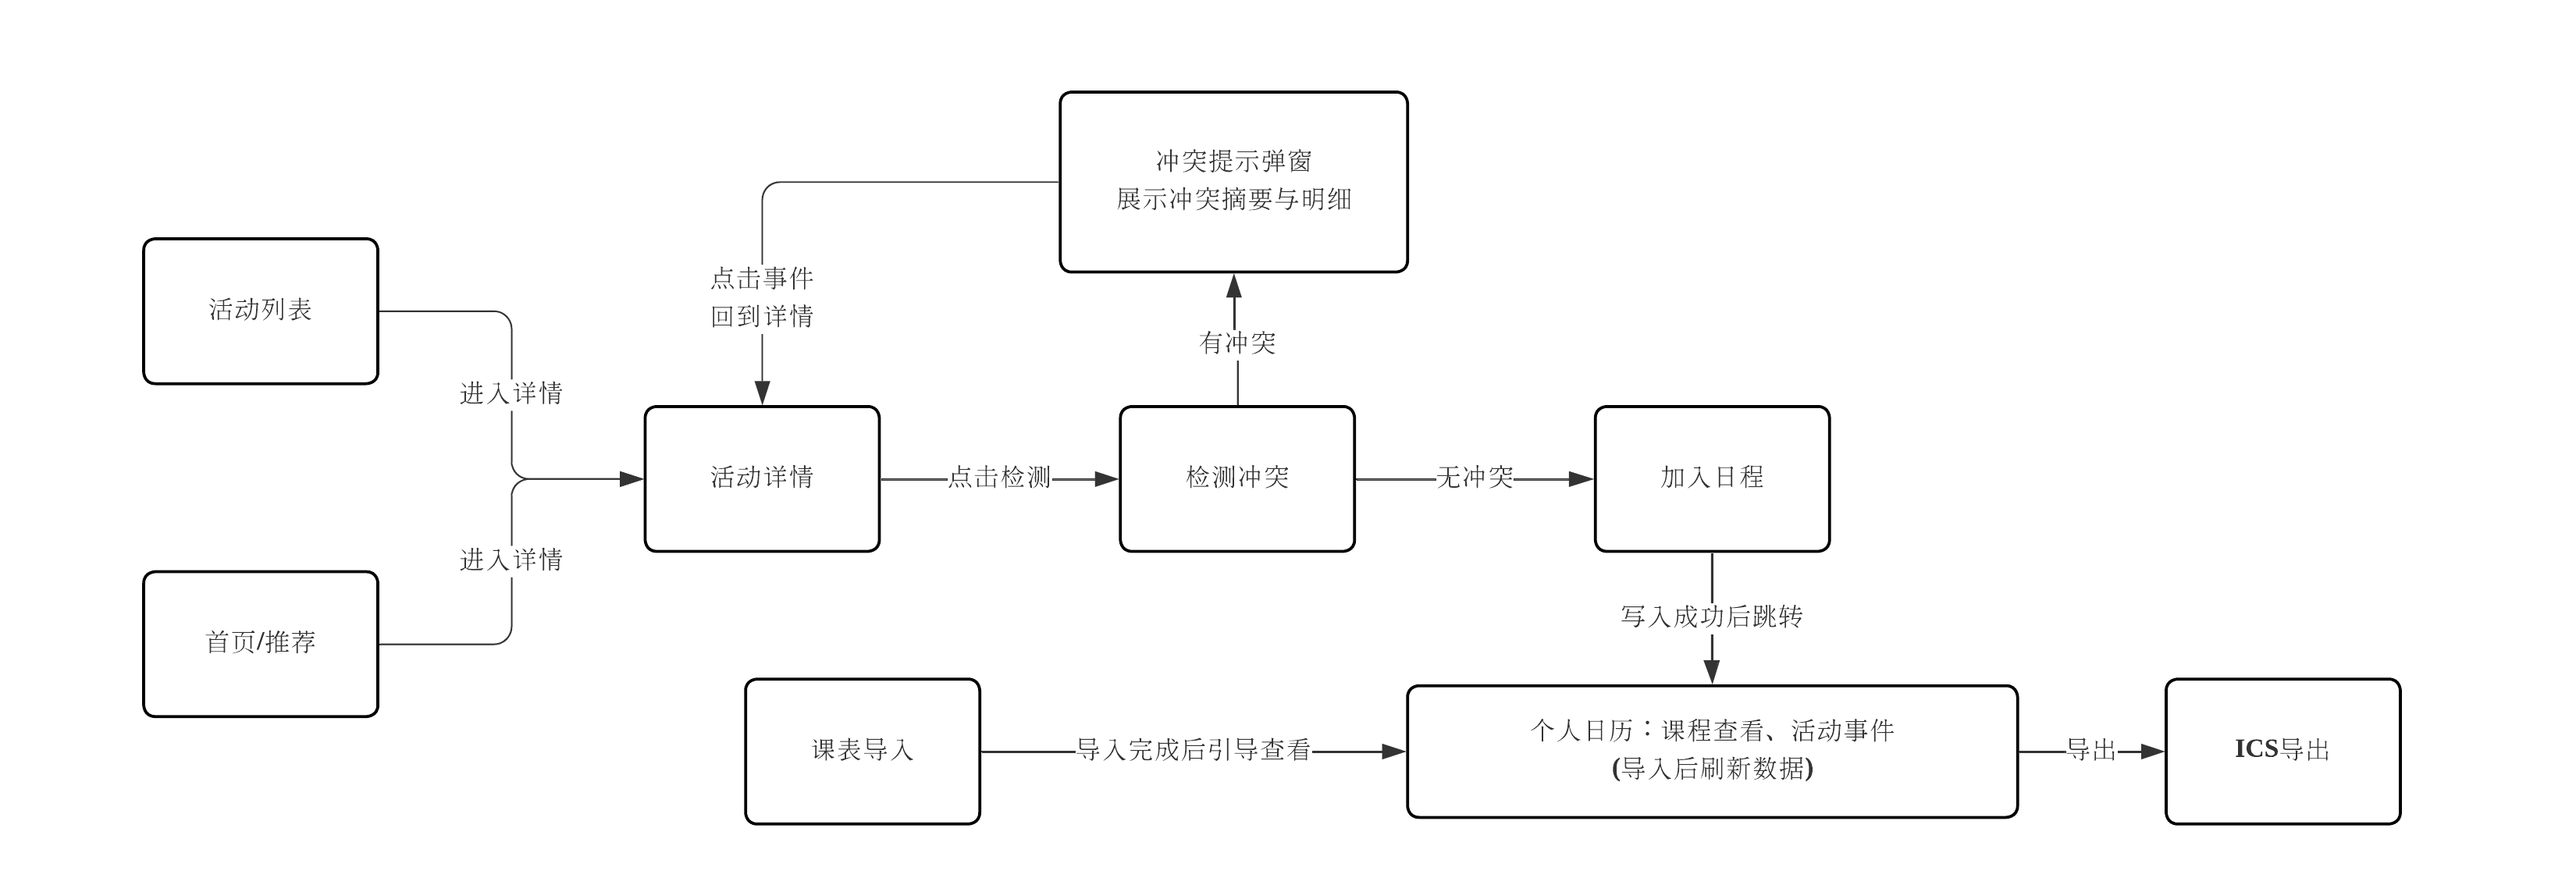
\includegraphics[width=0.96\linewidth,height=0.36\textheight,keepaspectratio]{3.4-0-ui-flow-overview.png}
    \vspace{0.5em}

    \begin{columns}[T,onlytextwidth]
        \begin{column}{0.46\textwidth}
            \begin{itemize}
                \item 首页和活动列表负责进入详情页
                \item 详情页展示时间、地点、标签和加入日程入口
                \item 日历页展示课程、活动和冲突提示
                \item 后台页维护活动数据和爬虫记录
            \end{itemize}
        \end{column}
        \begin{column}{0.50\textwidth}
            \centering
            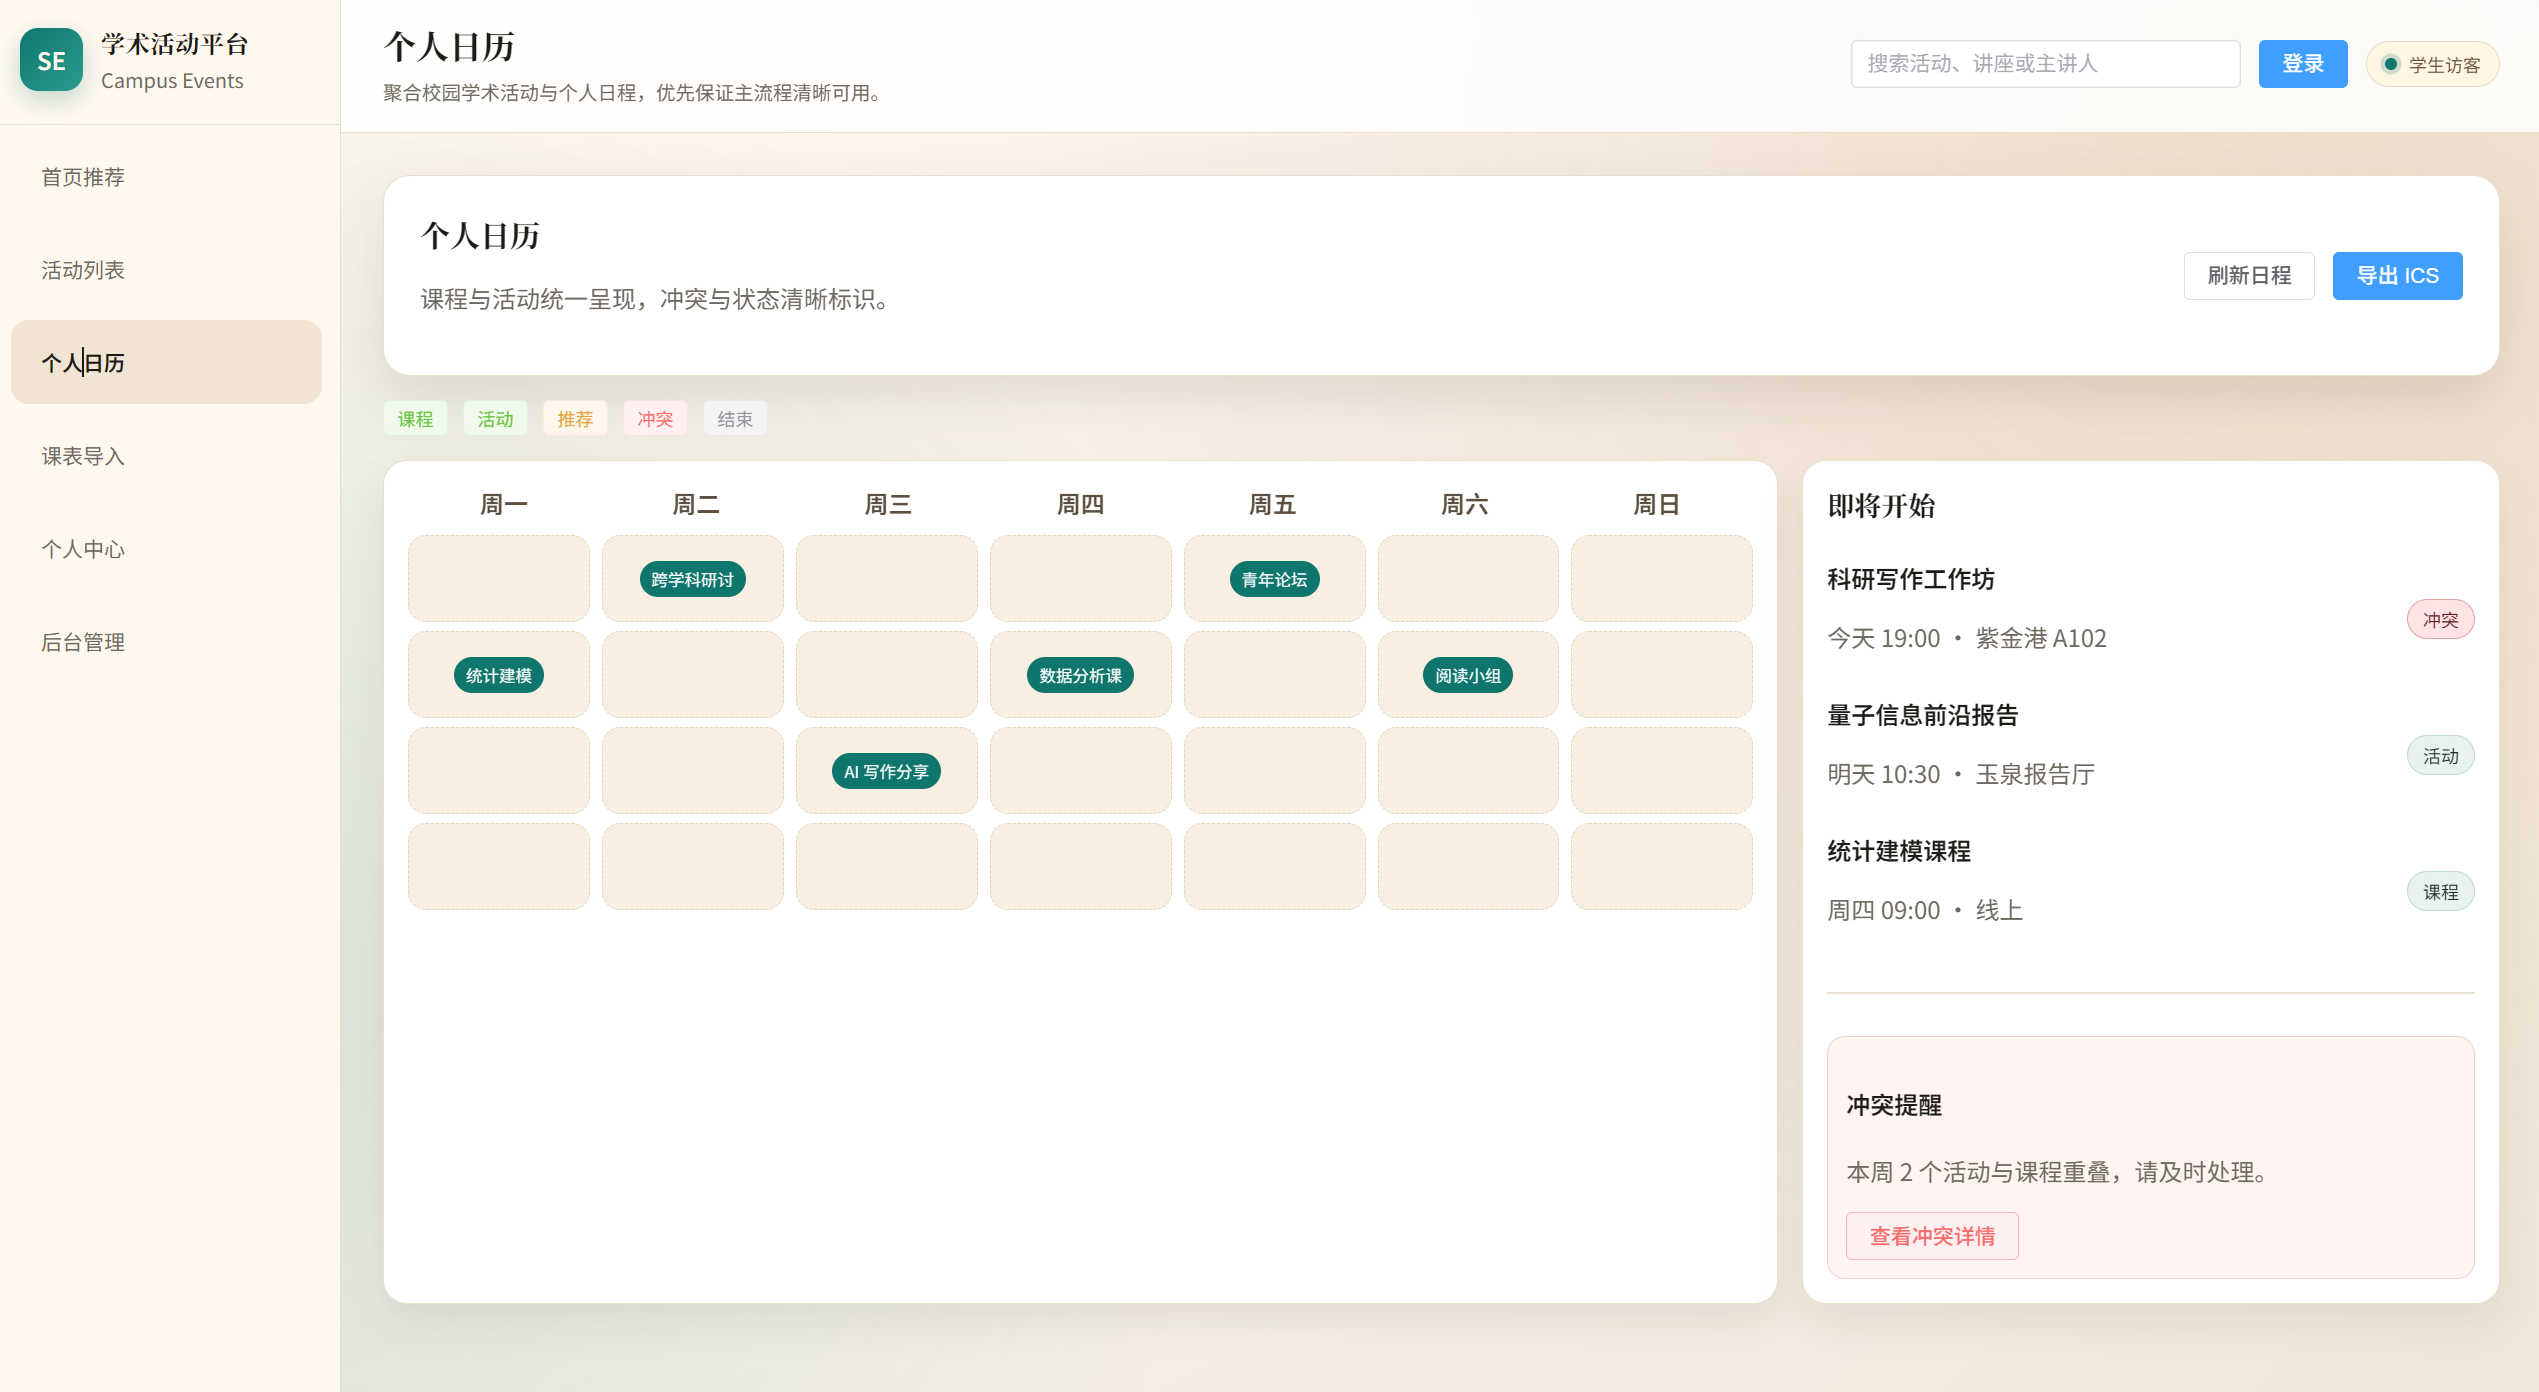
\includegraphics[width=\linewidth,height=0.28\textheight,keepaspectratio]{3.2-5-calendar.png}
        \end{column}
    \end{columns}
\end{frame}

\section{总结}
\begin{frame}{总结：预计交付产物与后续安排}
    \small
    \begin{columns}[T,onlytextwidth]
        \begin{column}{0.48\textwidth}
            \begin{block}{预计交付产物}
                \begin{itemize}
                    \item 可运行的 Web 系统：学生端页面与后台管理页
                    \item 后端接口：活动、推荐、课程、日程、认证和后台模块
                    \item 数据库脚本：表结构、测试数据和必要说明文档
                    \item 项目文档：接口文档、测试用例、用户手册和测试报告
                \end{itemize}
            \end{block}
        \end{column}
        \begin{column}{0.48\textwidth}
            \begin{block}{后续工作安排}
                \begin{enumerate}
                    \item 接入真实数据库，替换当前 mock 数据
                    \item 完成登录鉴权、管理员权限和活动维护流程
                    \item 实现搜索筛选、规则推荐、课表导入和冲突检测
                    \item 进行前后端联调，补充接口测试与演示数据
                \end{enumerate}
            \end{block}
        \end{column}
    \end{columns}
\end{frame}

\end{document}
